%!TeX root = ../main.tex

\section{COLMAP} \label{sec:COLMAP}
Having all the required files the performances of the compression system can be tested on a 3D-Reconstruction software, like COLMAP (\url{https://colmap.github.io/}). This software was meant for using SIFT features (see fig. \ref{fig:descriptors}), which are heavier and more performing in terms of quality but also less robust to image transformations (which must be accounted since the images are taken with a mobile phone) and patented. A trick that can be used is to use SURF features (64 float) and faking a larger dimensionality (128 float) by adding zeros. This way COLMAP recognizes the right dimensionality of the files while using SURF features instead of SIFT. In order to start the reconstruction, COLMAP will need three things:
\begin{enumerate}
\item A database to store the informations;
\item A set of images of the same scenario in different perspectives;
\item A .txt file for each image containing the features, in the format specified in sec. \ref{sec:FEATURES}. The title of the file must be the name of the image followed by .txt (\emph{e.g: image001.jpg.txt});
\item A .txt file containing the matchings between each image in the format specified in sec. \ref{sec:MATCHINGS}.
\end{enumerate}
Not having these will result in an error inside COLMAP which won't start the reconstruction.


\begin{figure}[h!]
    \centering
    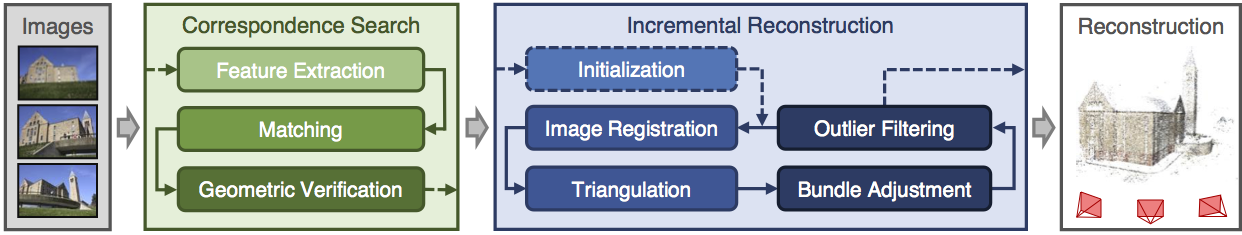
\includegraphics[width=\textwidth]{images/colmap.png}
    \caption{COLMAP’s incremental SfM pipeline.}
    \label{fig:colmap}    
\end{figure}